
\subsection{Term unfolding for homogeneous inputs}
\label{sec:homo-unfold}

\subsubsection{Preliminaries}

\paragraph*{Partial shallow unfold}
 If $\rGamma$ and $\rDelta$ are types, we define $\ranked{\Gamma\odot\Delta}$ to be $\ranked{\Gamma.(\Delta+\set{1})}$. We call its inhabitants the \emph{partial shallow} terms. A partial shallow term looks like this, where we omitted to draw the element $1$ 
\begin{center}
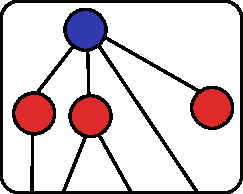
\includegraphics[scale=.4]{partial-shallow-term.pdf}
\end{center}
We define the \emph{partial shallow unfolding} function as the extension  of the shallow unfold function of Figure~\ref{fig:weak-unfolding} to partial shallow terms. It is the function of type 
\begin{align*}
\ranked{{\reduce k \Sigma}\odot{\Gamma^k} \to \reduce k ({\Sigma}\odot{\Gamma})} 
\end{align*}
defined as in the following picture
 \begin{center}
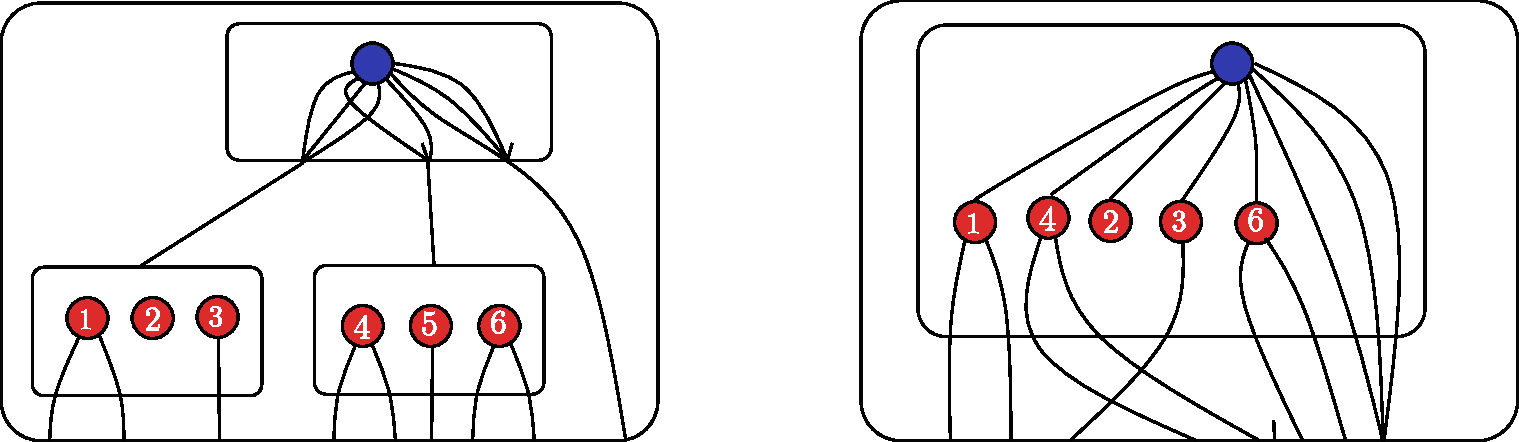
\includegraphics[scale=.4]{partial-shallow-unfold.pdf}
 \end{center}
the partial shallow unfolding function can be derived as follows. Consider the functions $\ranked{f}$ and $\ranked{g}$ defined as follows
\begin{align*}
\ranked{f:\Gamma^k \xrightarrow{\text{Increse-fold}} \reduce k  \Gamma^k \xrightarrow{\reduce k (\iota_1)^k} \reduce k  (\Gamma+1)^k}  \\ 
\ranked{g:1 \xrightarrow{\text{k-Unit}} \reduce k 1^k \xrightarrow{\reduce k (\iota_2)^k} \reduce k  (\Gamma+1)^k }
\end{align*}
We start by lifting $f$ and $g$ as follows
\begin{align*}
\ranked{\reduce k \Sigma \odot \Gamma^k\overset{\text{{\tiny def}}}{=} \reduce k \Sigma \cdot (\Gamma^k+1) \to  \reduce k \Sigma \cdot \reduce k (\Gamma+1)^k}
\end{align*}
We compose the obtained function with the prime function which distributes   the shallow product over the fold:
\begin{align*}
\ranked{\reduce k \Sigma \cdot \reduce k (\Gamma+1)^k \to \reduce k (\reduce k \Sigma \cdot (\Gamma+1)^k)}
\end{align*}
Now we can apply the shallow unfold function, more precisely we lift it along the constructor $\reduce k$. Then we compose the result with the product of the graded monad:
\begin{align*}
\ranked{\reduce k (\reduce k \Sigma \cdot (\Gamma+1)^k) \xrightarrow{\reduce k \text{Shallow unfold}} \reduce k \reduce 1 ( \Sigma \cdot (\Gamma+1)) }
\end{align*}
Then we compose the result with the product of the graded monad, to obtain the desired function
\begin{align*}
\ranked{\reduce k \reduce 1 (\Sigma \cdot (\Gamma+1)) \xrightarrow{\flatt} \reduce k \Sigma \cdot (\Gamma+1) \overset{\text{{\tiny def}}}{=} \reduce k \Sigma \odot \Gamma}
\end{align*}

\paragraph*{Term unfolding for constant-twist inputs}

We say that a term $ t \in \tmonad \mati k \rSigma$ is a \emph{constant-twist term}  if each twist of an internal branches is a constant function. Note that the internal twists need not to be the same constant function. Here is an example of a constant-twist term

  \begin{center}
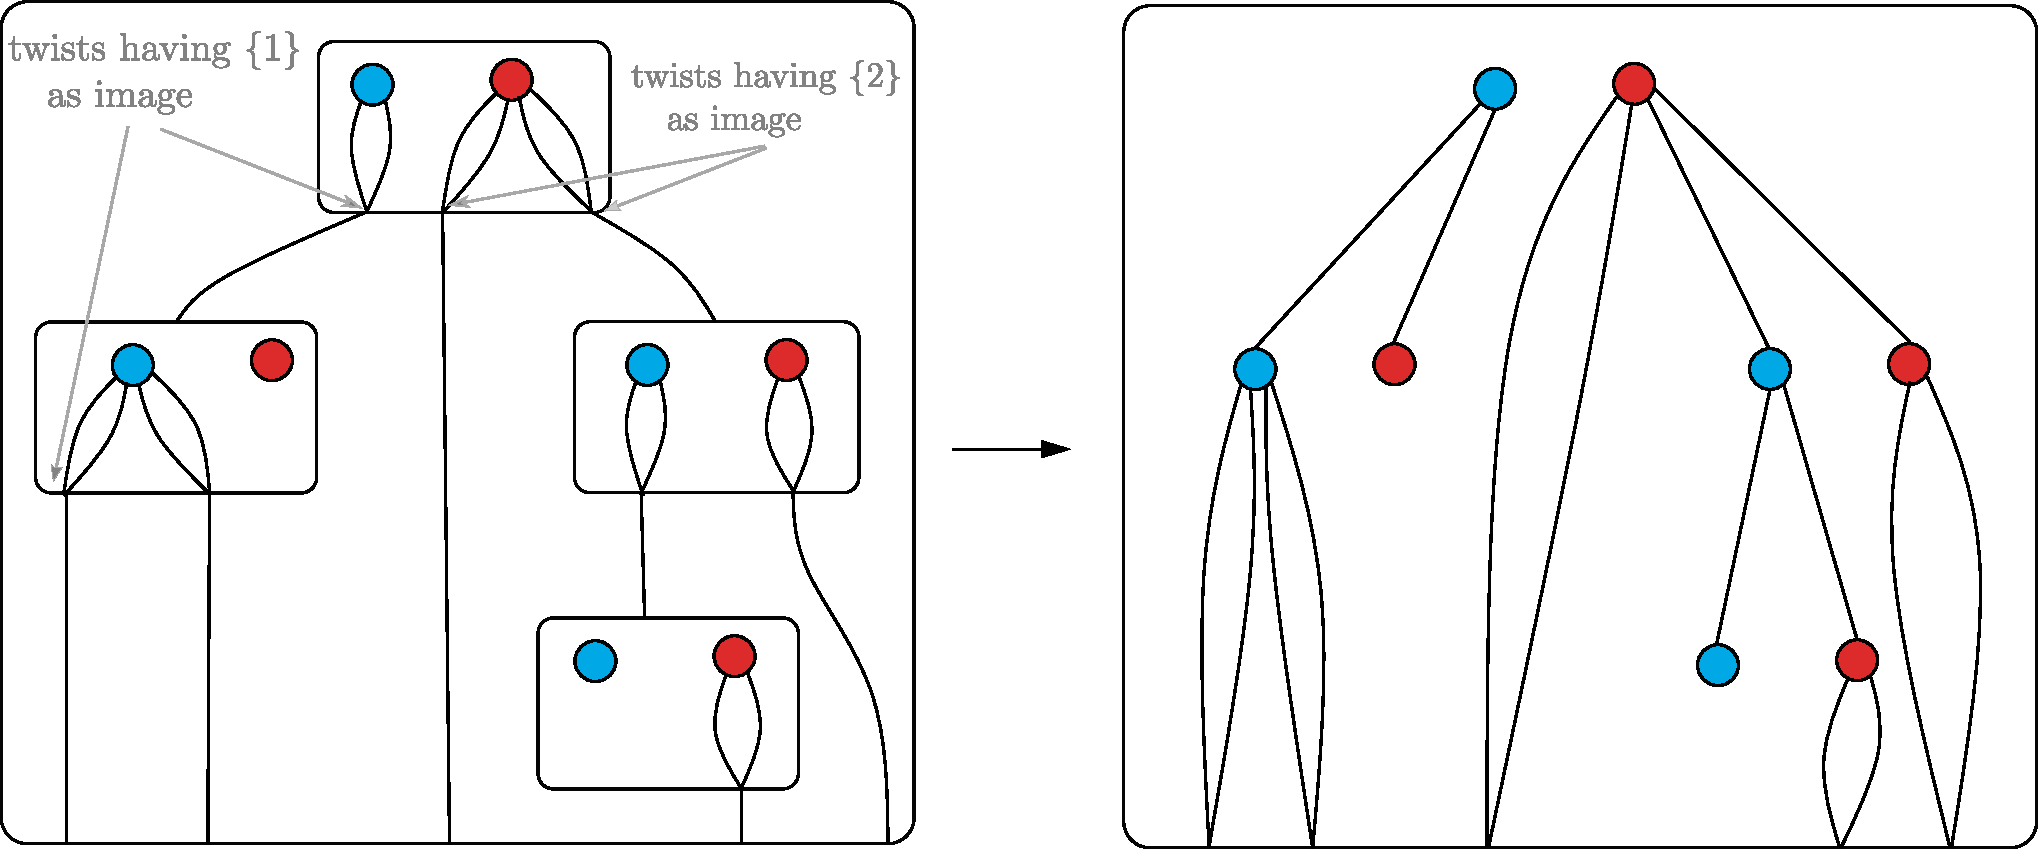
\includegraphics[scale=.35]{one-unfold.pdf}
 \end{center}
 This section is devoted to proving the following lemma. 

\begin{lemma}\label{lem:constant-twist}
    Let $k \in \set{1,2,\ldots}$. There is a derivable function 
    \begin{align*}
        \ranked{f : \tmonad \mati k \rSigma \rightharpoonup \mati k {(\tmonad \Sigma)} }
        \end{align*}      
which coincides with unfolding for all constant-twist inputs.
\end{lemma}

\begin{proof}
The function $f$ can be derived using the following steps. We use the example of the constant-twists term above as a running example.  
\begin{enumerate}
\item We start by applying the external unfolding function.  We get a term in $\ranked{\reduce k \tmonad \Sigma^{[k]}}$. Our example becomes like this
   \begin{center}
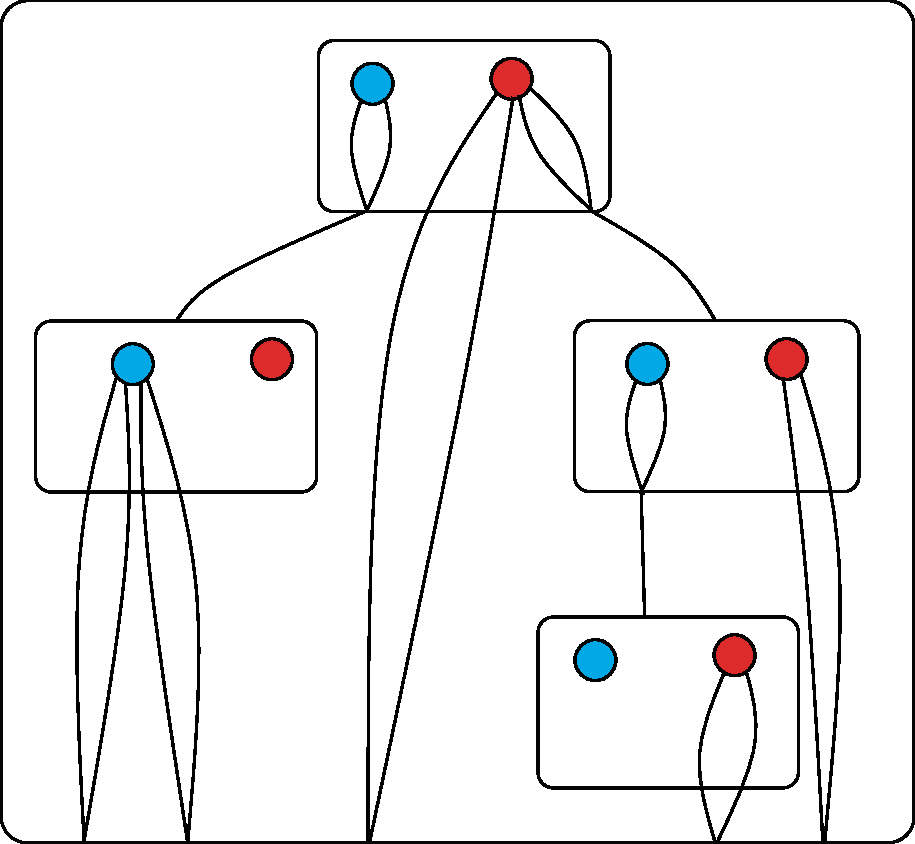
\includegraphics[scale=.35]{one-unfold1.pdf}
 \end{center}
 \item Next, we will transform each matrix power node into a tensor product as follows 
 \begin{align*}
 \ranked{ \Sigma^{[k]} \rightarrow \reduce k (\reduce k \Sigma \otimes \dots \reduce k \Sigma) \to \reduce 1 (\reduce k \Sigma)^k}
 \end{align*}
 The idea here is that, since the image of each twist is a singleton,  the ports of the matrix power are independent. We can then transform safely each node into a tensor product. After that, we transform each tensor product $\ranked{(\reduce k \Sigma)^k}$ into a shallow term $\ranked{k.\reduce k \Sigma}$ which we see itself as a term of type $\ranked{\tmonad(k+\reduce k\Sigma)}$. After the application of the unfolding function $\mathrm{unfold}_1$ followed by a flattening, and the simplification of $\ranked{\reduce k \reduce 1 \tmonad (k+\reduce k \Sigma)}$ into $\ranked{\reduce k \tmonad (k+\reduce k \Sigma)}$ we get a term in $\ranked{\reduce k \tmonad(k+\reduce k \Sigma)}$. Our running example becomes as follows after this step
   \begin{center}
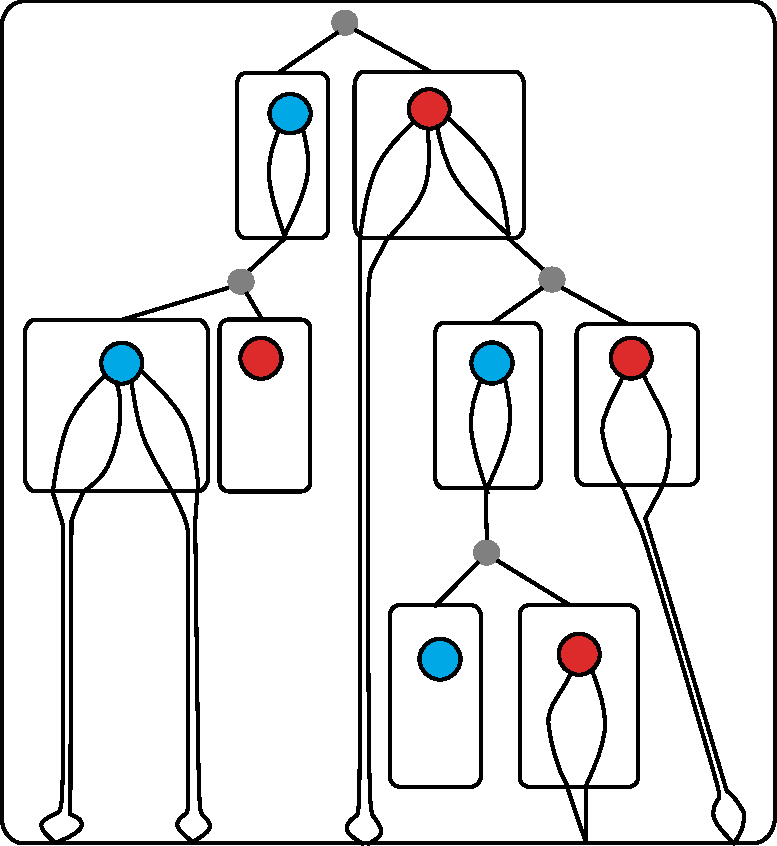
\includegraphics[scale=.35]{one-unfold2.pdf}
 \end{center}
 \item Now we apply the factorization 
 \begin{align*}
 \ranked{\tmonad (k + \reduce k \Sigma)\to \tmonad \tmonad(k + \reduce k \Sigma)}
 \end{align*}
 which regroups each element $\ranked{\reduce k \Sigma}$ with its children of type $\ranked{k}$ in the same factor, and leaves the other nodes in isolated factors. At this point our term looks like this
   \begin{center}
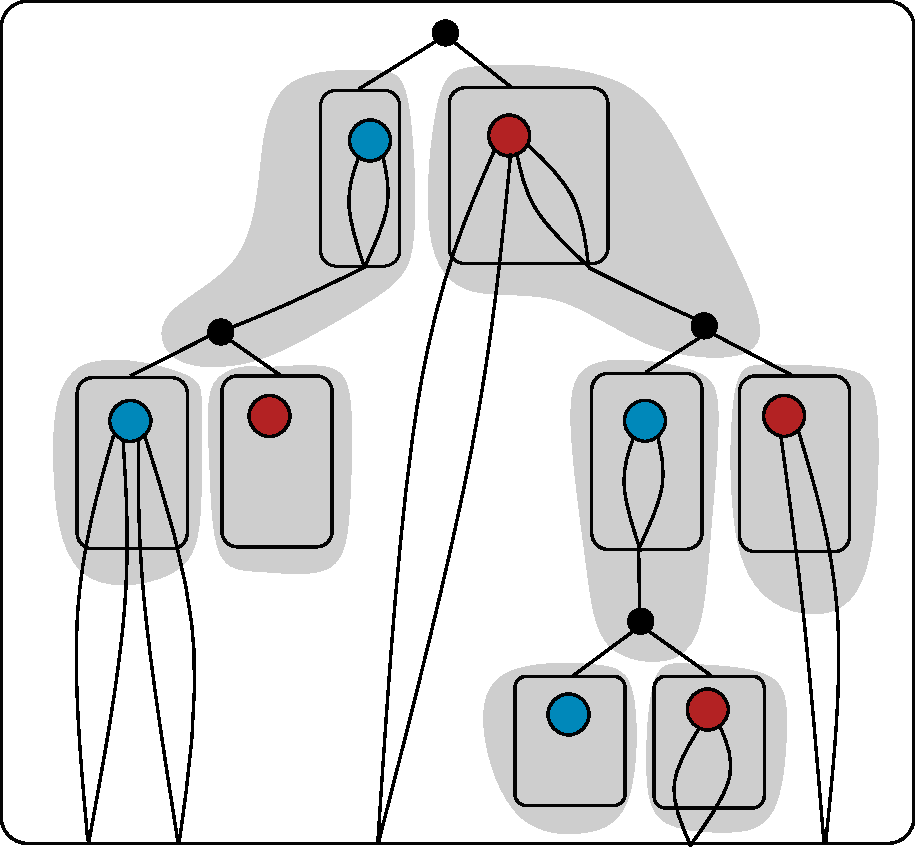
\includegraphics[scale=.35]{one-unfold3.pdf}
 \end{center}
 Note that this factorization have the following shape: the root is labeled by $k$, and all the other nodes have labels in $\ranked{(\reduce k \Sigma) \odot k}$. We want to reflect this structure in  the type by applying the following function
 \begin{align*}
 \ranked{\tmonad \tmonad(k + \reduce k \Sigma) \to k. \tmonad ((\reduce k \Sigma)\odot k)}
 \end{align*}
 This function can be implemented easily using the decomposition function, the functions which maps every type to $\ranked{1}$ and mechanisms of raising errors. 
 \item In each node $\ranked{(\reduce k \Sigma)\odot k}$, we transform $\ranked{k}$ into $\ranked{1^k}$ (this function is basic since its domain is finite). After that, we apply the partial shallow unfold function, composed with the prime functions eliminating the $1$ and decreasing the fold:
\begin{align*}
\ranked{(\reduce k \Sigma)\odot k \to \reduce k (\Sigma \odot 1) \to \reduce k \Sigma \to \reduce 1 \Sigma}
\end{align*} 
  as illustrated by the following picture
   \begin{center}
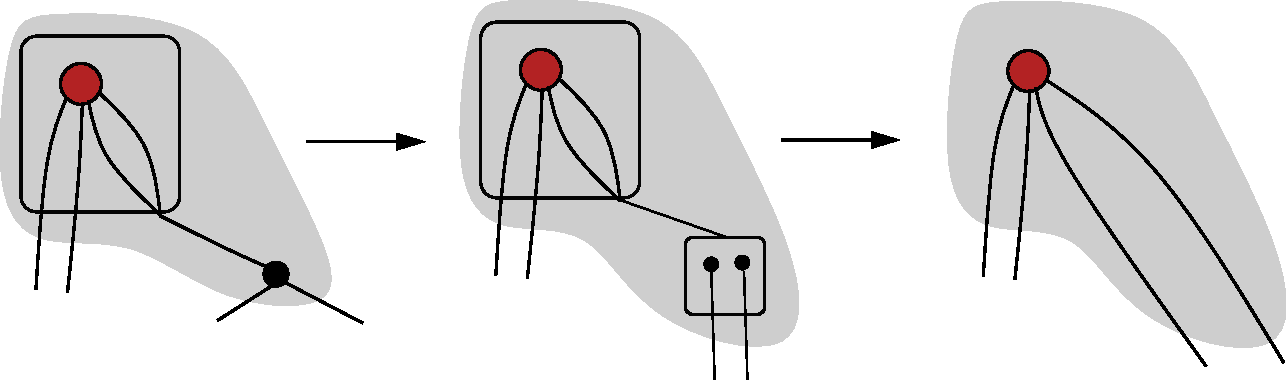
\includegraphics[scale=.3]{one-unfold4.pdf}
 \end{center}
 \item At this point we have a term of type $\ranked{\reduce k (k\cdot \tmonad \reduce 1 \Sigma)}$. We apply the untwist function
 \begin{align*}
 \ranked{\tmonad \reduce 1 \Sigma \to \reduce 1 \tmonad \Sigma}
 \end{align*}
 then the function which transforms shallow terms into tensor product
 \begin{align*}
 \ranked{k \cdot \reduce 1 \tmonad \Sigma \to (\reduce 1 \tmonad \Sigma)^k}
 \end{align*}
 Now our term is of type $\ranked{\reduce k (\reduce 1 \tmonad \Sigma)^k}$. To conclude, we apply the prime function which permutes the tensor product with the fold, then we apply the product of the graded monad. 
 \end{enumerate}
\end{proof}

\subsubsection{Term unfolding for $\alpha$-homogeneous inputs}
\label{subsec:alpha-homo-unfold}

For a monotone function 
\begin{align*}
\alpha: \set{1,\ldots,k} \to \set{1,\ldots,k}
\end{align*}
we say that a term $ t \in \tmonad \mati k \rSigma$ is $\alpha$-homogeneous if all internal branches have twist $\alpha$. This section is devoted to proving the following lemma. 

\begin{lemma}\label{lem:homo-twist}
    Let $k \in \set{1,2,\ldots}$ and let $\alpha : \set{1,\ldots,k} \to \set{1,\ldots,k}$ be a monotone function. There is a derivable operation 
    \begin{align*}
        \ranked{f : \tmonad \mati k \rSigma \to \mati k {(\tmonad \Sigma)} }
        \end{align*}      
which coincides with term unfolding for all inputs which are $\alpha$-homogeneous.
\end{lemma}

\begin{proof}
We proceed by induction on $k$. When $k=1$, the unfolding coincides with the basic distributivity function 
\begin{align*}
\ranked{ \tmonad \reduce 1 \Sigma \to {\reduce 1 \tmonad \Sigma}}
\end{align*}
Let us treat the inductive case. For that, we introduce a tool that will be useful to analyze the function $\alpha$. For a function $$\alpha: \set{1,\ldots,k} \to \set{1,\ldots,k}$$ define  \emph{its graph} as the directed graph whose set of vertices is $\set{1,\ldots,k}$, and which contains an edge $i\rightarrow j$ if $\alpha(i)=j$. Note that the out-degree of the nodes is $1.$

\medskip
In the proof of the inductive case, we distinguish two cases. The first one is when the graph of $\alpha$ is not weakly connected. In this case, by monotonicity of $\alpha$, we can find $m\in \set{1,k-1}$ such that $\alpha(\set{1,m})\subseteq\set{1,m}$ and $\alpha(\set{m+1,k})\subseteq\set{m+1,k}$. The idea is then to create two copies of the original term: in the first one we keep only the first $m$ elements of the tensor product of each node, and in the second one we keep the last $k-m$ copies. Then we unfold these terms by applying the induction hypothesis, and  finally we gather them to obtain the  unfolding of the original term. 

%\smallskip
%To illustrate this case, we consider the following function $\alpha$, whose graph is shown below
%\begin{center}
%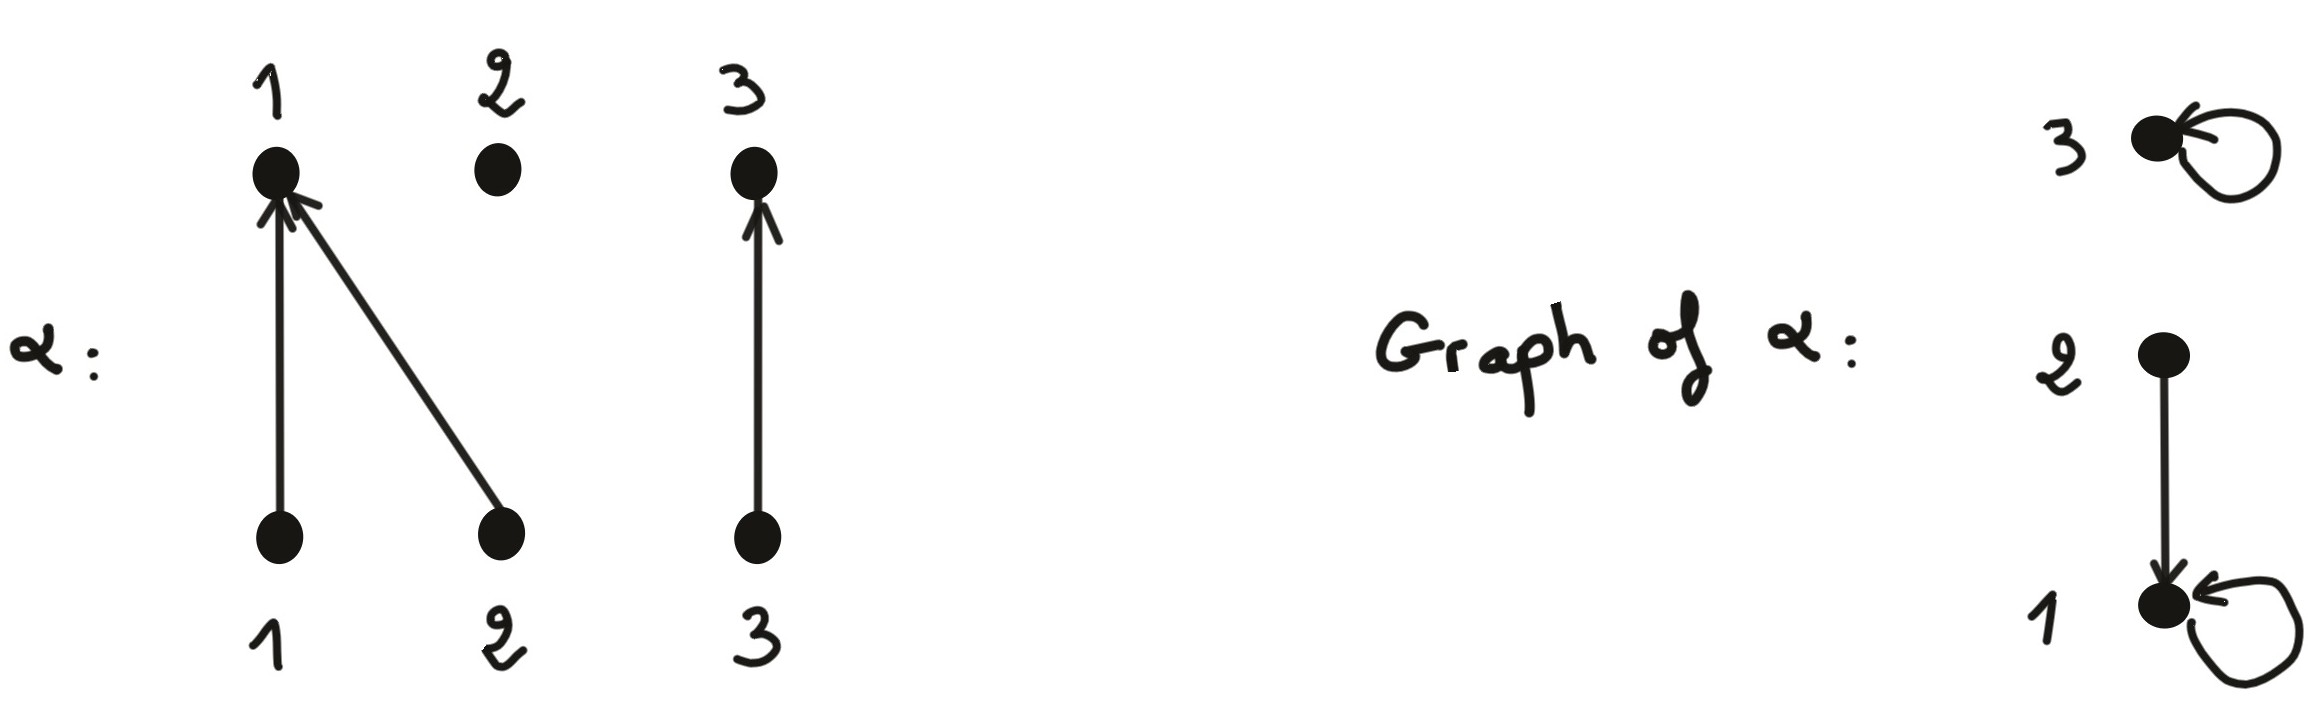
\includegraphics[scale=.07]{MyPic27.jpg}
%\end{center}
%The graph of $\alpha$ is not weakly connected: it contains two weakly connected components, $\set{1,2}$ and $\set{3}$.
%Consider the following $\alpha$-homogeneous terms $t$ of $\tmonad \mati k \rSigma$ which will be our running example in the not weakly connected case of the proof. We colored in blue the elements of the first weakly connected part of the graph of $\alpha$ and in green the second part.
%\begin{center}
%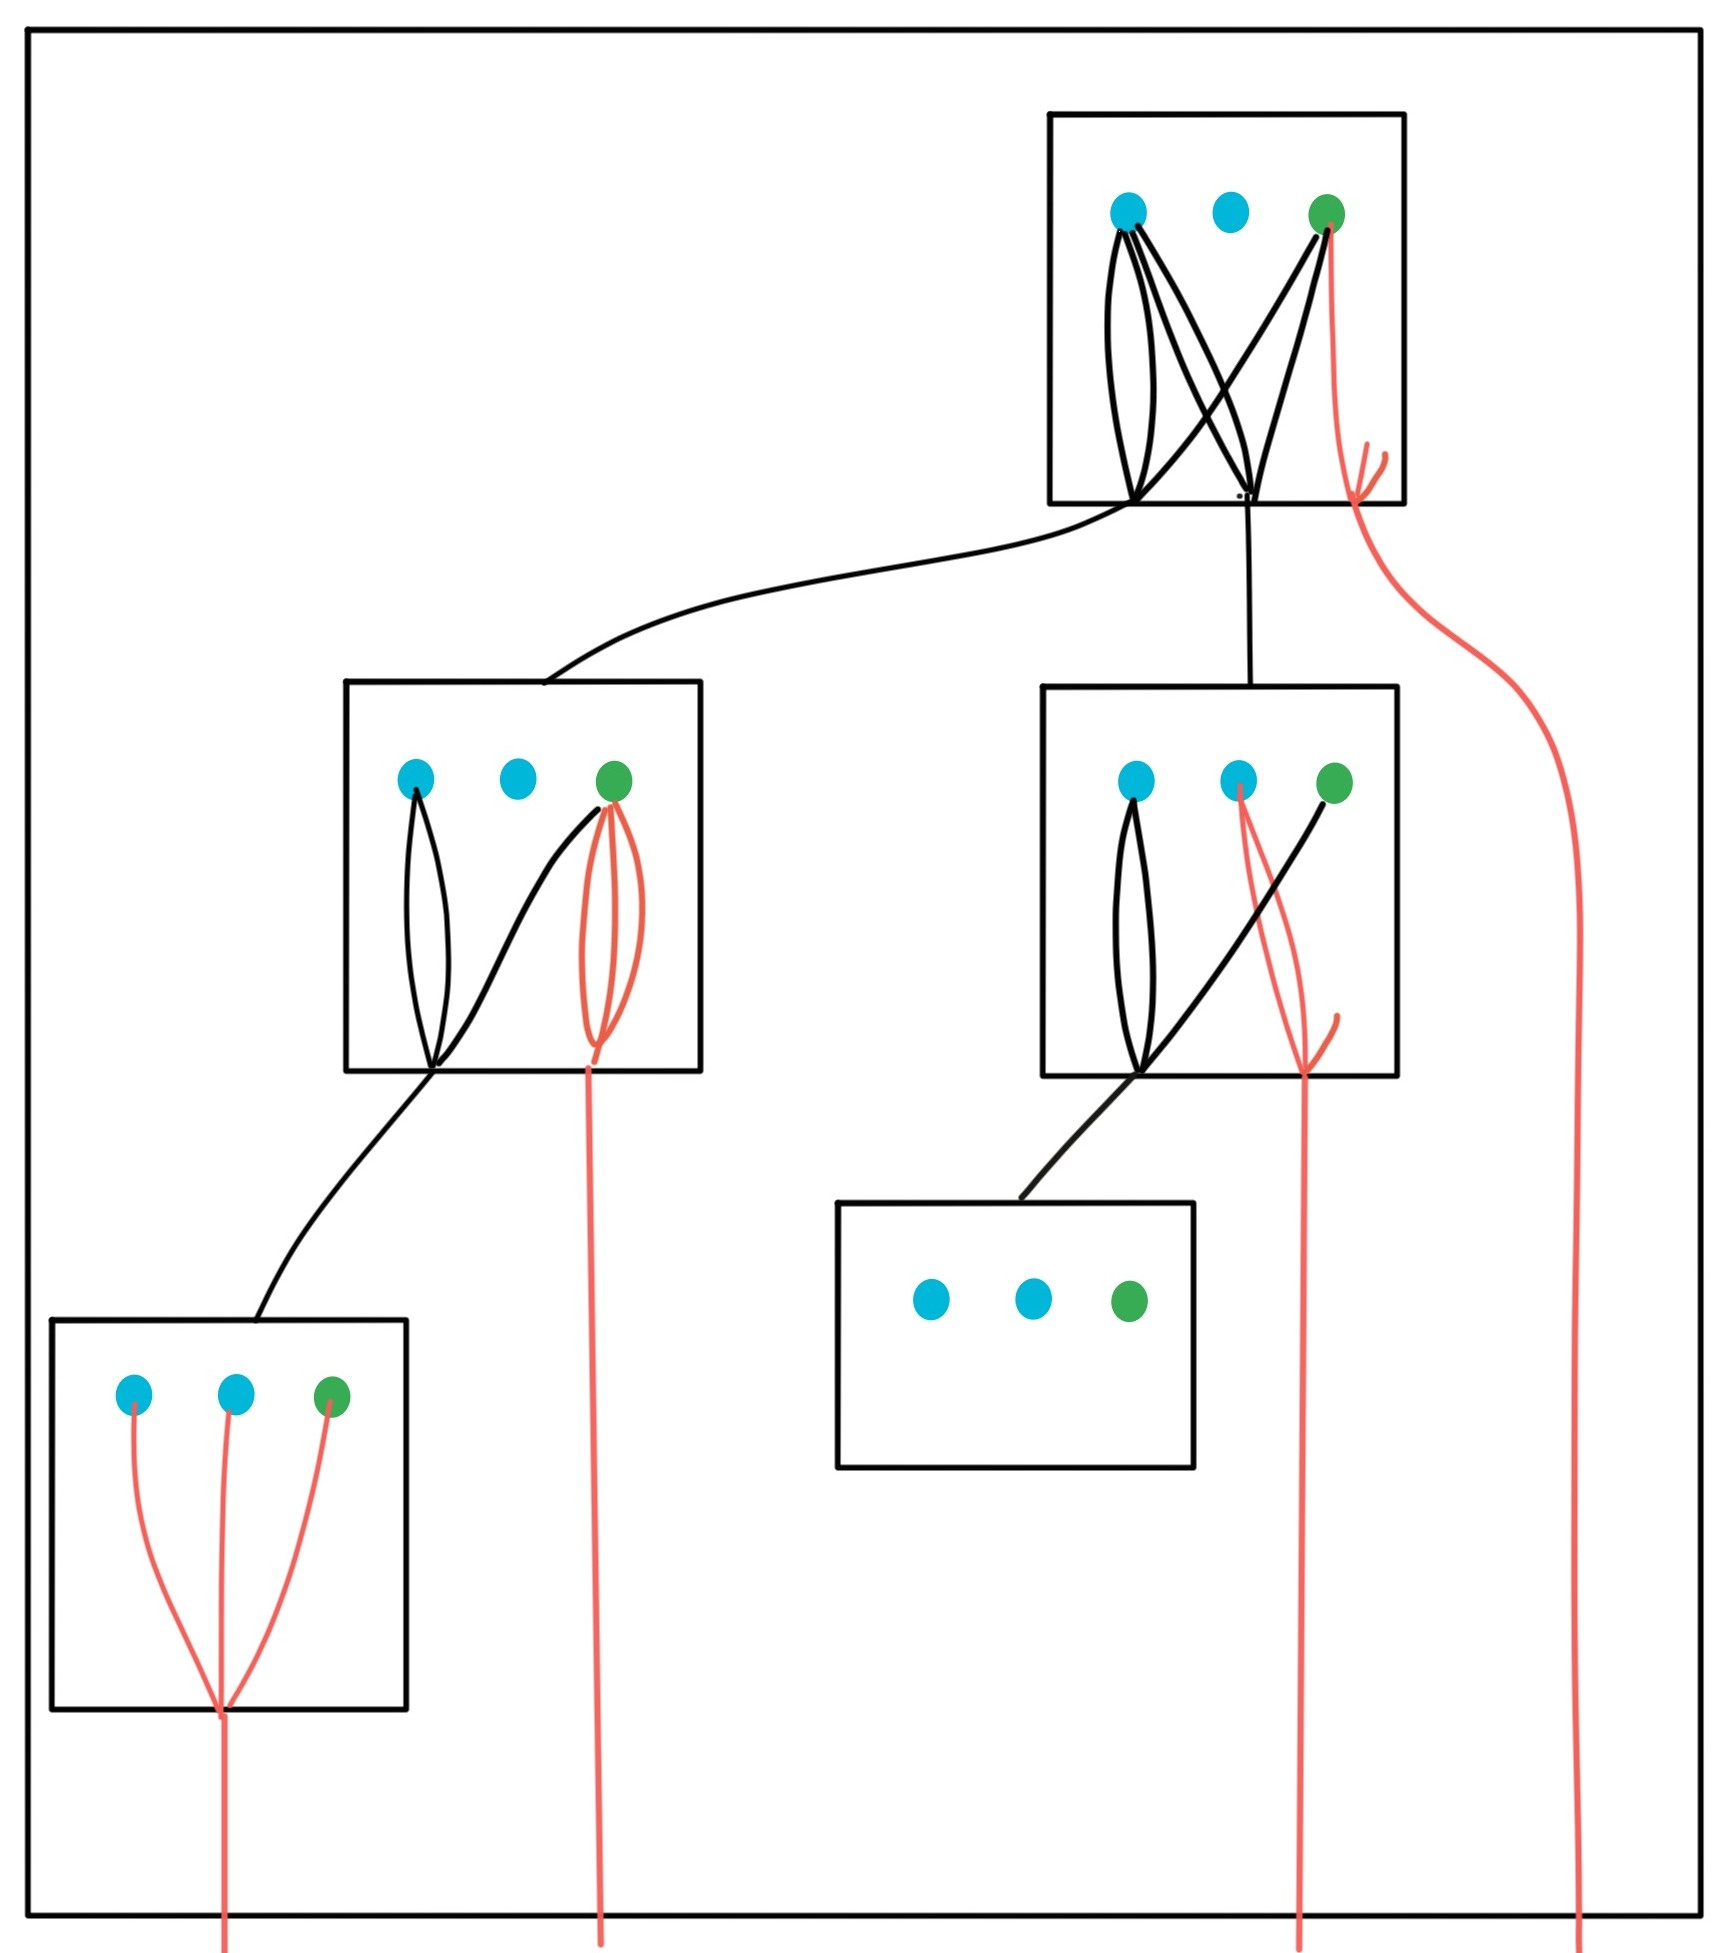
\includegraphics[scale=.07]{MyPic28.jpg}
%\end{center}
Let us now implement the ideas we discussed above. We start by unfolding the external twists, using the basic external unfold function. This way, the domain of every external twist  cannot be shared by the two disconnected components of the domain of $\alpha$.
%Our running example becomes like this:
%\begin{center}
%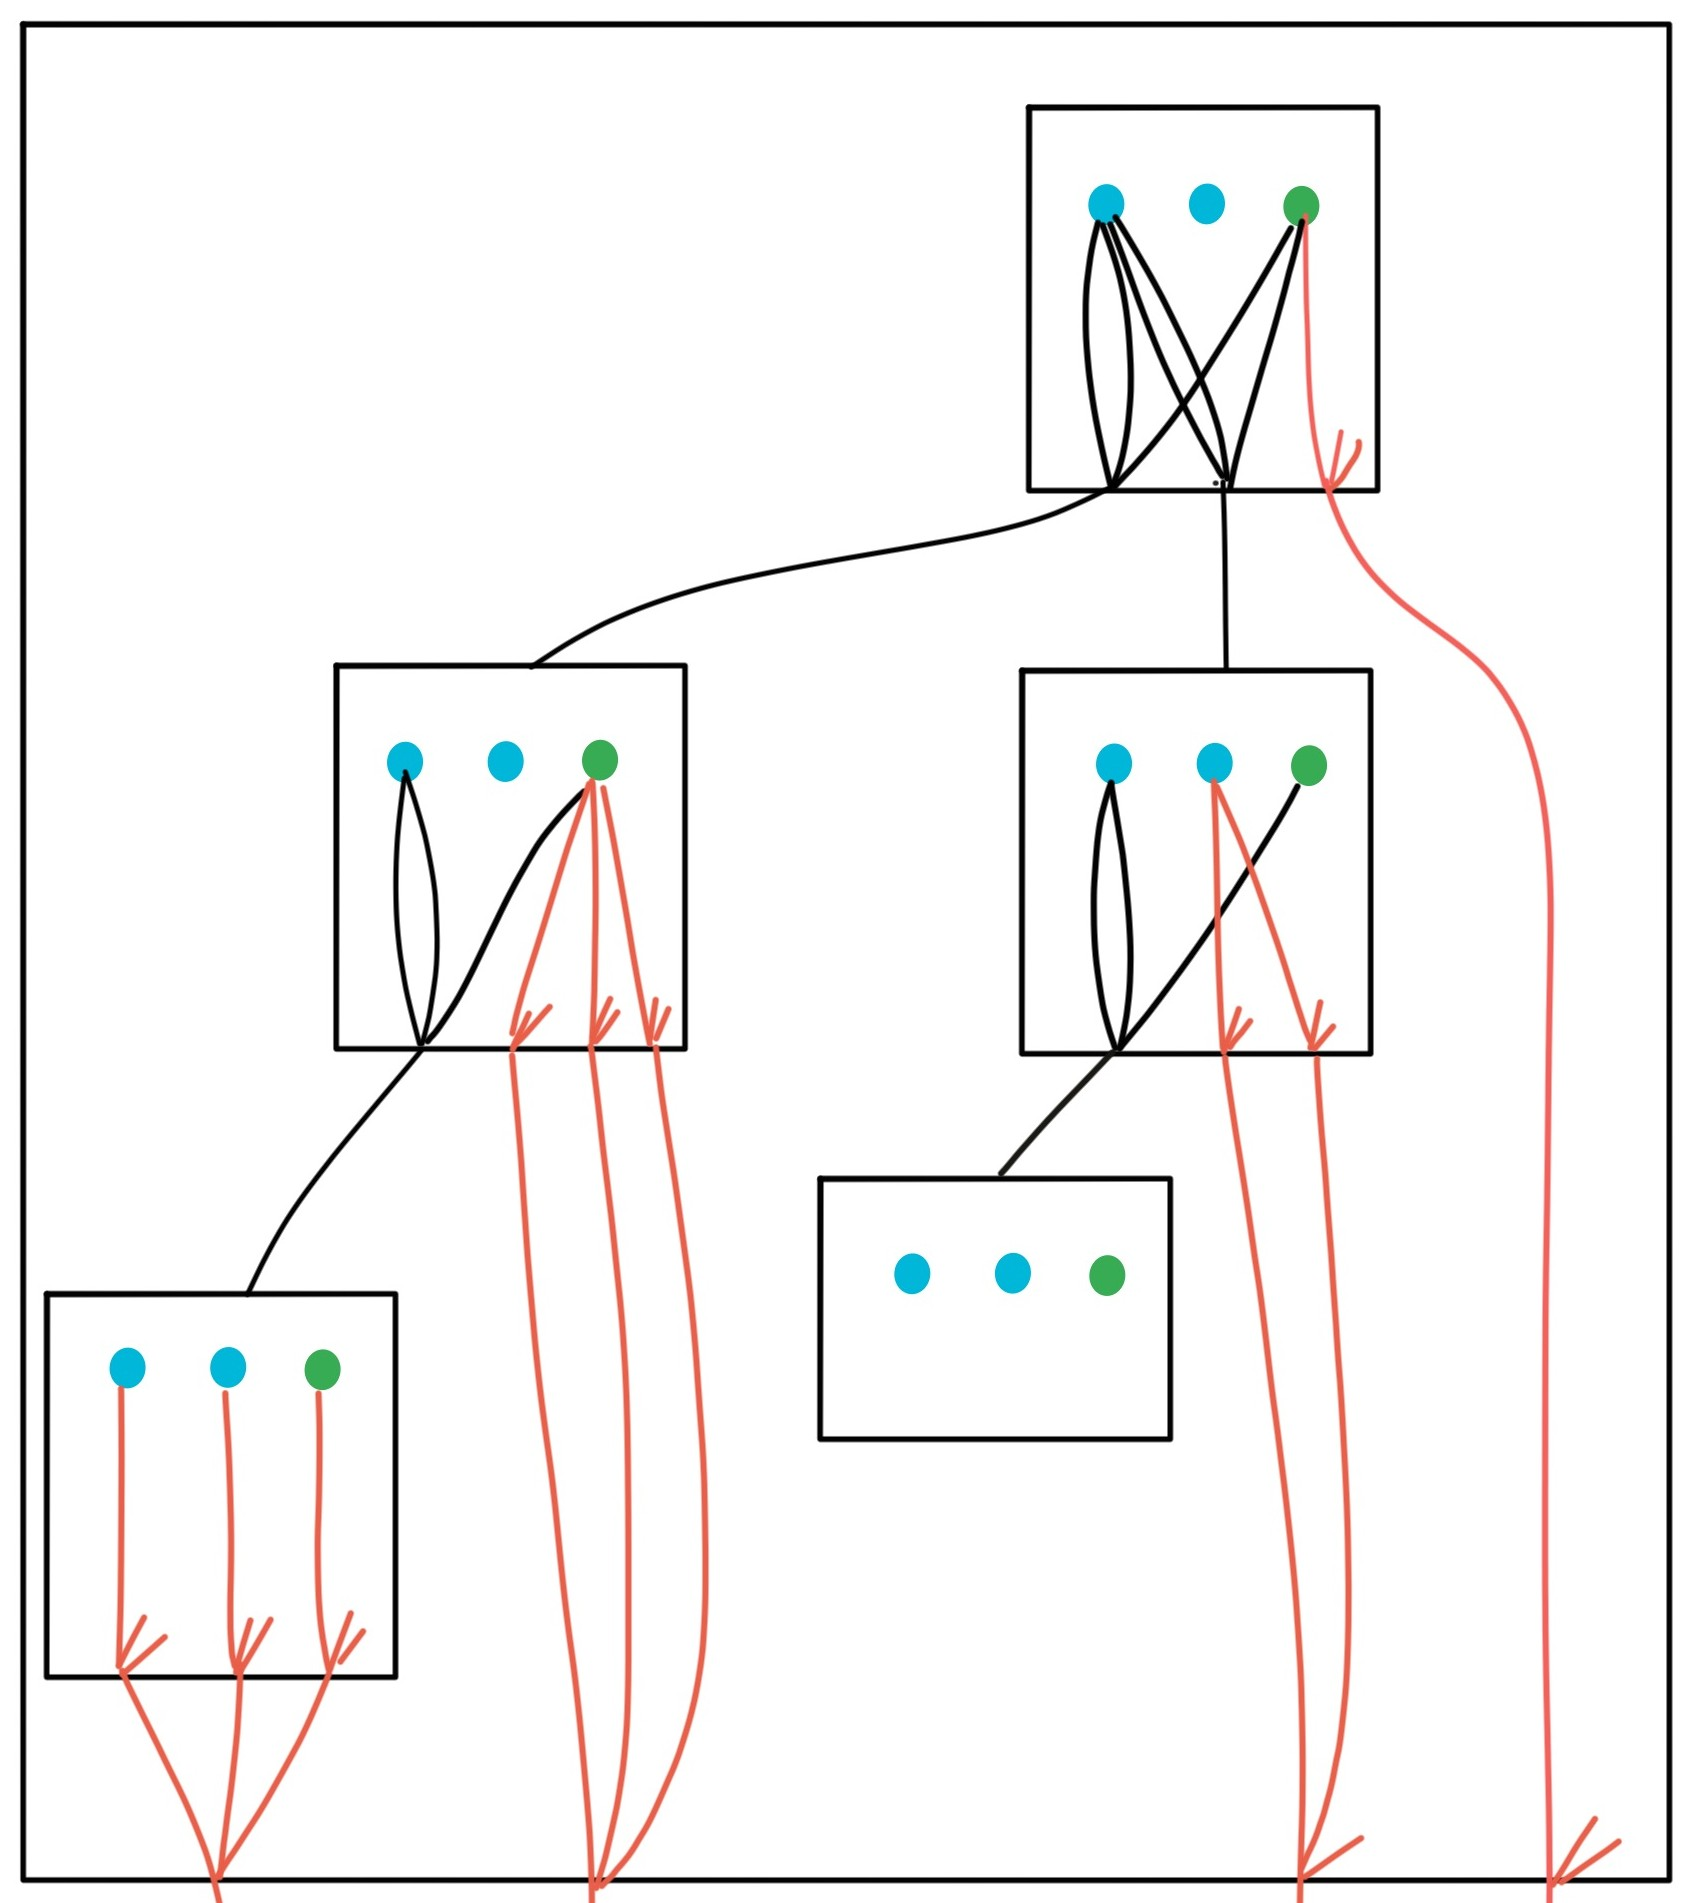
\includegraphics[scale=.07]{MyPic29.jpg}
%\end{center}
Then, we duplicate the input term using the basic function 
\begin{align*}
\ranked{\tmonad \mati k \Sigma\to \reduce 2 (\tmonad \mati k \Sigma\otimes \tmonad \mati k \Sigma)}
\end{align*}
To the first copy, we apply the function  
\begin{align*}
\ranked{f_1:\tmonad \mati k \Sigma \to \mati m {(\tmonad \Sigma)}}
\end{align*}
which keeps only the first $m$ elements of the tensor product, then applies the induction hypothesis to the obtained term.
To the second copy, we apply the function 
\begin{align*}
\ranked{f_2:\tmonad \mati k \Sigma \to \mati {k-m} {(\tmonad \Sigma)}}
\end{align*}
which keeps only the last $k-m$ elements of the tensor product, then applies the induction hypothesis to the obtained term.

%Here is the effect of the functions $f_1$ and $f_2$ on our example
%\begin{center}
%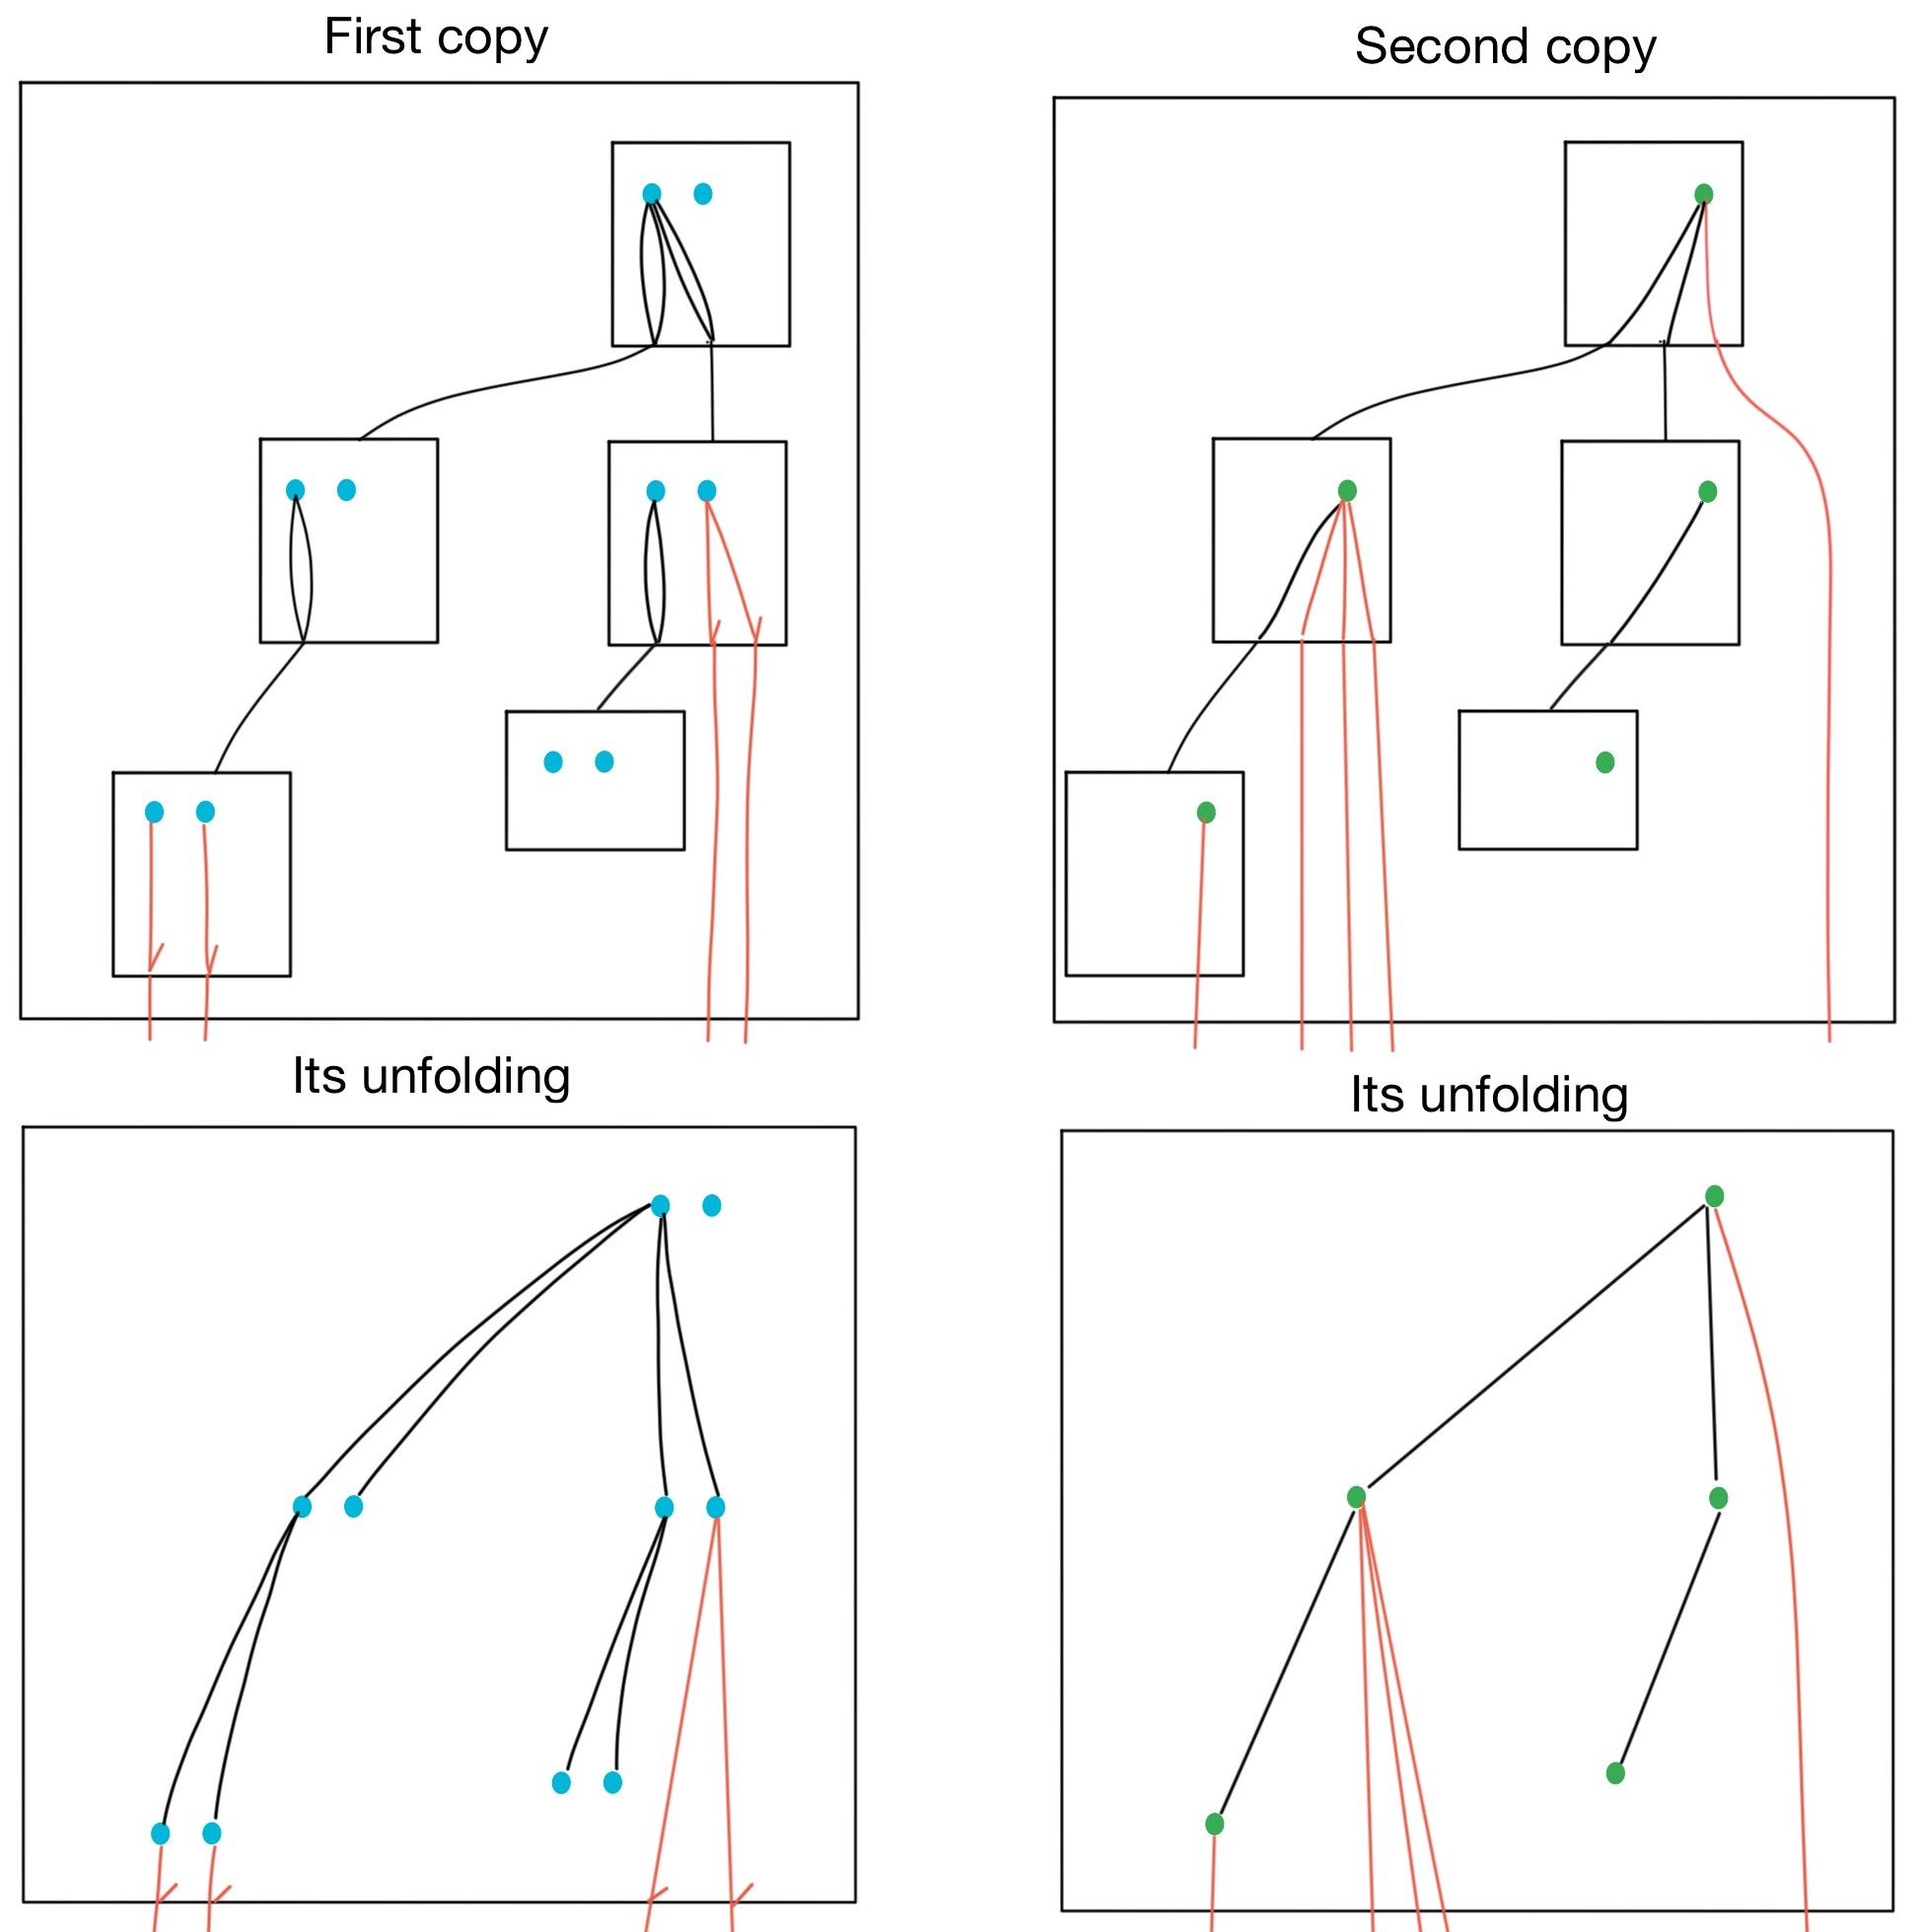
\includegraphics[scale=.15]{MyPic30.jpg}
%\end{center}
 The function $\ranked{f_1}$ can be derived using the tensor projection function, the merge of folds, then reducing the fold and finally invoking the induction hypothesis. 
%\begin{align*}
%\begin{prooftree}
%\Hypo{\overbrace{\ranked{\mati k \Sigma \to \reduce k \reduce 1 \Sigma^m}}^{\substack{\text{Lift the projection on the first}\\\text{$m$ elements of the tensor to $\reduce k$}}}}
%\Hypo{\overbrace{\ranked{\reduce k \reduccomponenetse 1 \Sigma^m \to \reduce k \Sigma^m}}^{\substack{\text{Merge the folds $\reduce k$ and $\reduce 1$}}}}
%\Hypo{\overbrace{\ranked{\reduce k \Sigma^m \to \mati m {(\Sigma\cdot (1+0))}}}^{\substack{\text{Adjust the degree of the fold}\\\text{to get a matrix power}}}}
%\Infer{3}[]{\ranked{\mati k \Sigma \to \mati m {(\Sigma\cdot (1+0))}}}
%\end{prooftree}
%\end{align*}


When we apply $\ranked{f_1}$ and $\ranked{f_2}$ to the two copies of the original term, we get a term of type 
\begin{align*}
\ranked{ \reduce 2 (\mati m {(\tmonad \Sigma)}\otimes  \mati {k-m} {(\tmonad\Sigma)})}
\end{align*}
%Now, we need to get the fold outside the tensor product. For that, we lift both $\ranked{\mati m {(\tmonad \Sigma)}}$ and $\ranked{\mati {k-m} {(\tmonad \Sigma)}}$ to $\ranked{\reduce k (\tmonad \Sigma)^m}$ and $\ranked{\reduce k (\tmonad \Sigma)^{k-m}}$ respectively. Then we commute the fold with the tensor product using the following basic function:
%\begin{align*}
%\ranked{\reduce k (\tmonad \Sigma)^m\otimes\reduce k (\tmonad \Sigma)^{k-m}\to \reduce k (\tmonad \Sigma)^k}
%\end{align*}
%Then we merge the two  folds $\reduce 2$ and $\reduce k$ into $\reduce {2k}$. After these operations, we get the desired term, but not with the desired type (the type we get is $\ranked{\reduce {2k} (\tmonad\Sigma)^k}$). To get the right type, which is $\ranked{\mati k {(\tmonad\Sigma)}}$, we apply the  function which reduces the degree of the fold
%\begin{align*}
%\ranked{\reduce {2k} (\tmonad \Sigma)^k \to \reduce {k} (\tmonad \Sigma)^k}
% \end{align*}
% The term we get for our example is the following, which is the unfolding of the original term
% \begin{center}
% 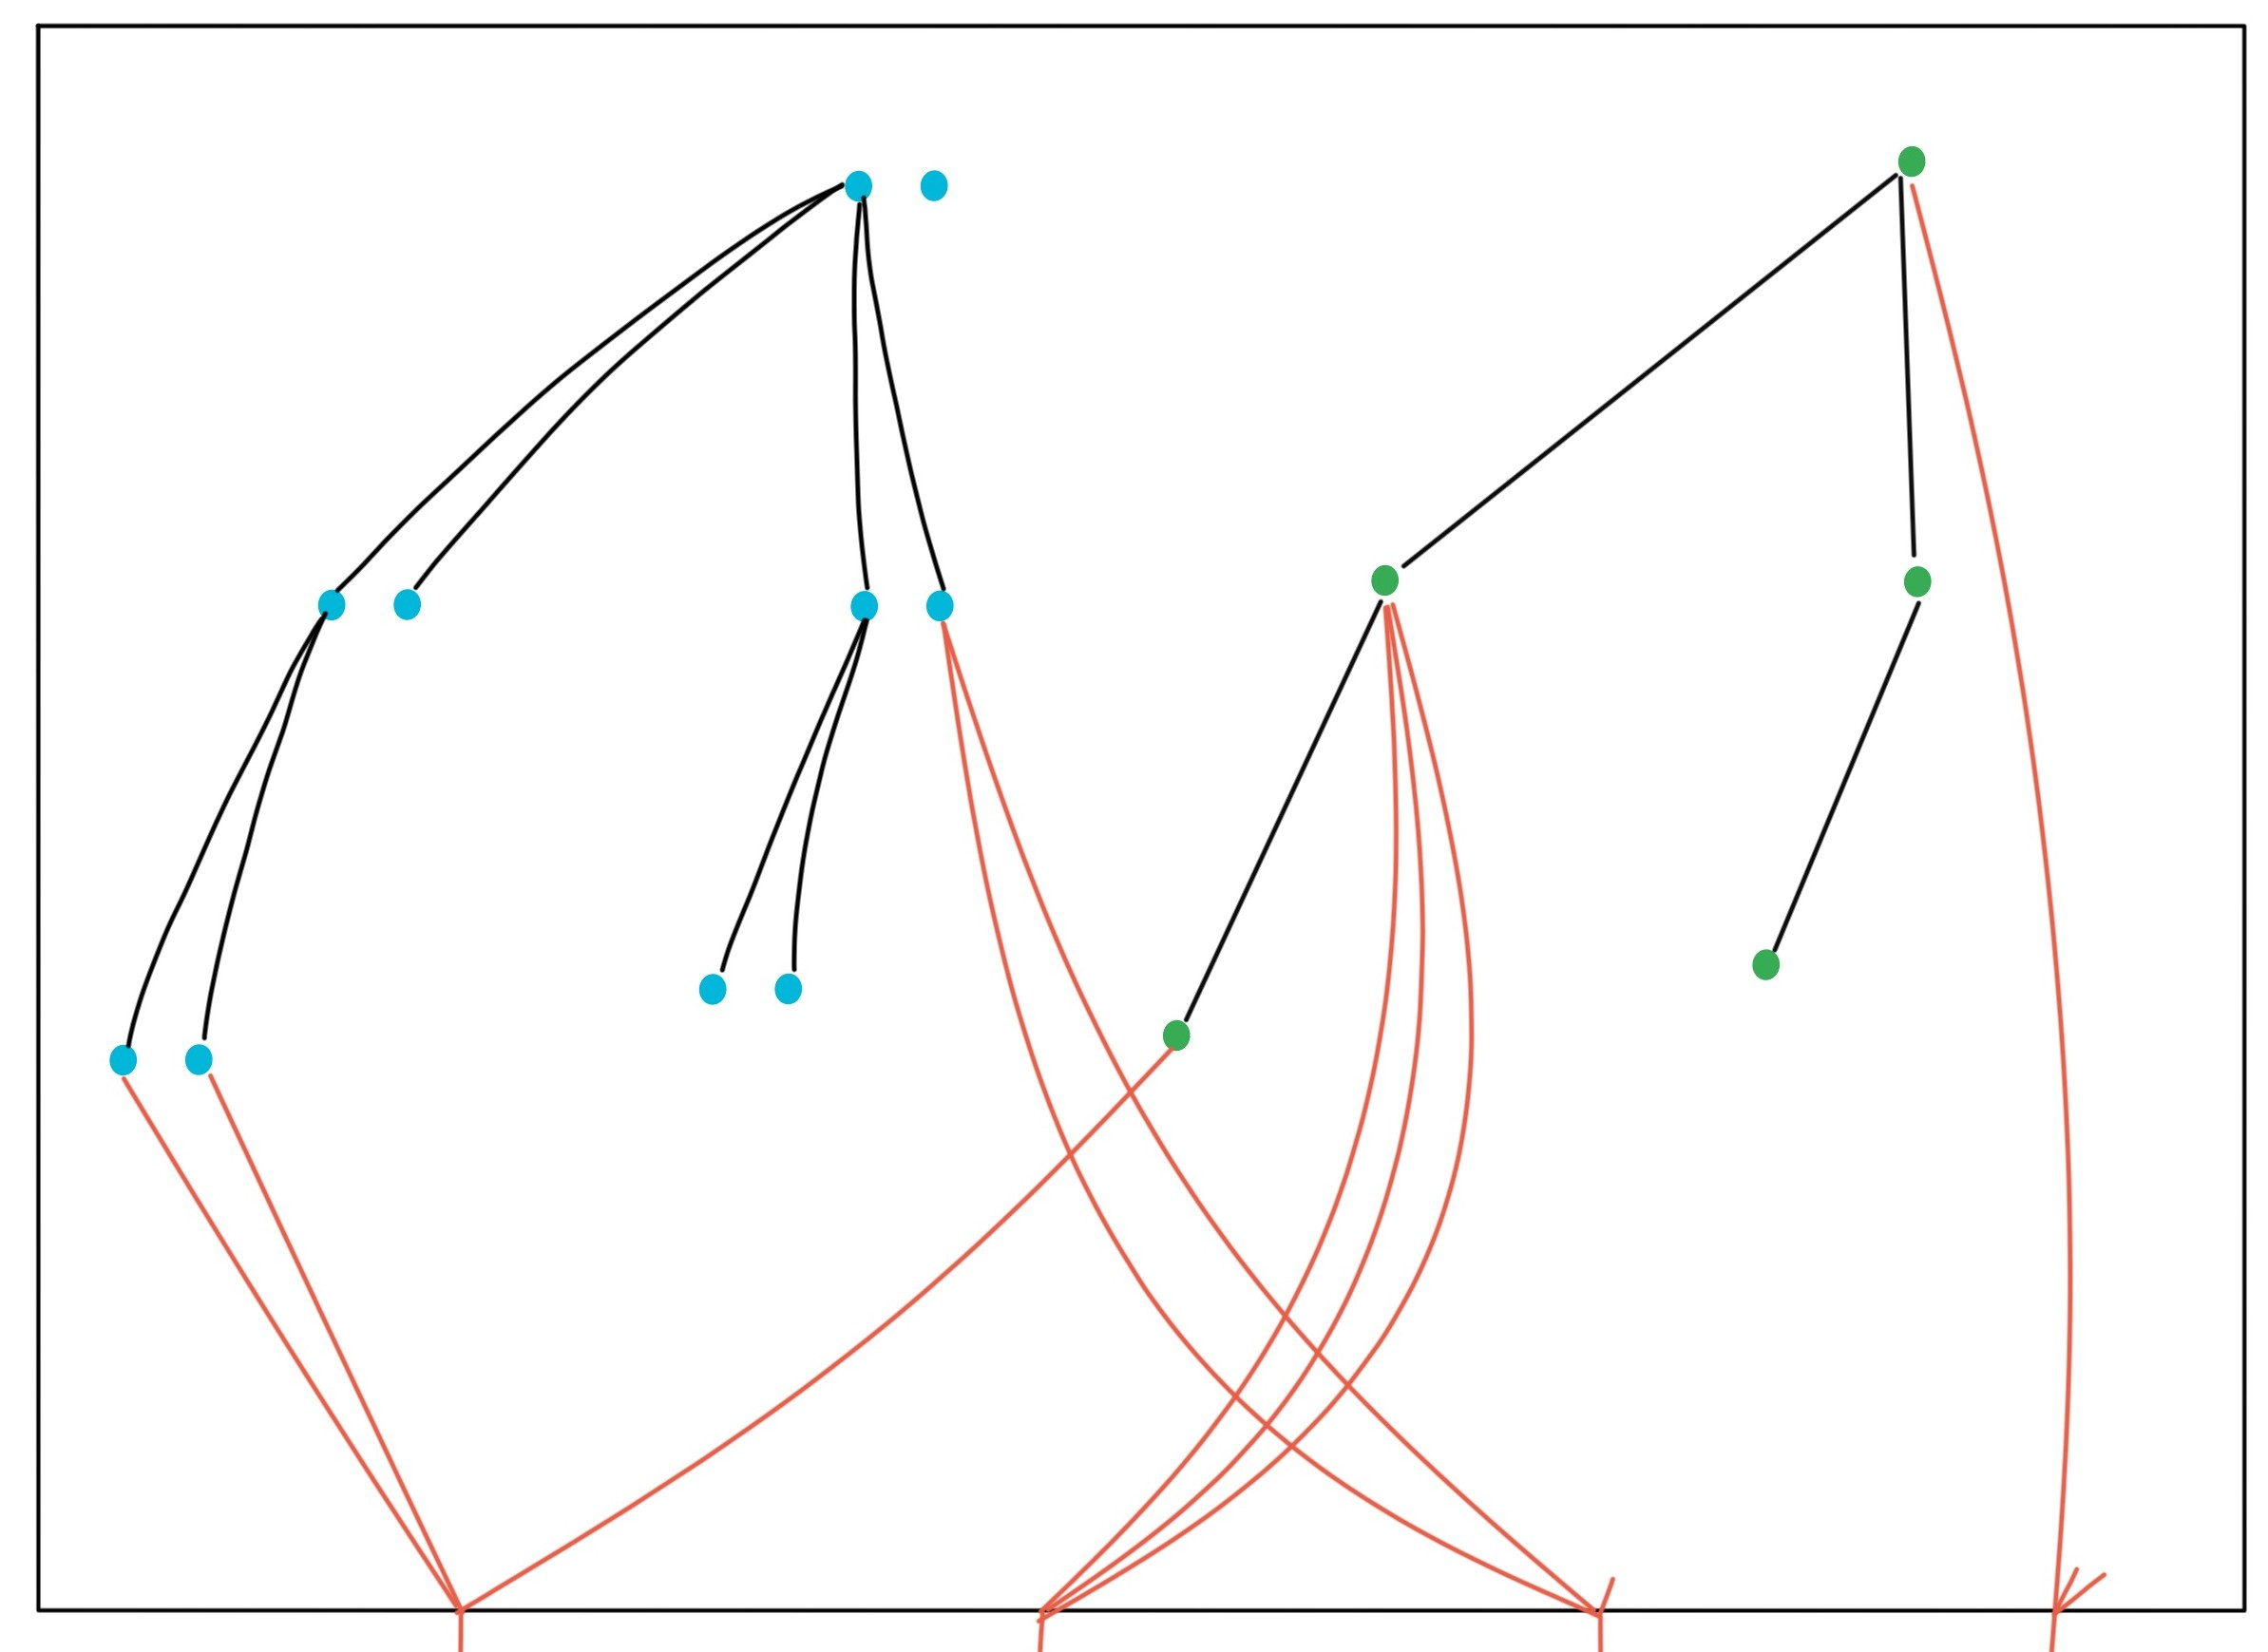
\includegraphics[scale=.08]{MyPic31.jpg}
% \end{center}
At this point, we are almost done, we only need to transform the type in order to match the desired type. For that we increase the fold by applying the following prime functions
\begin{align*}
\ranked{\reduce m (\tmonad \Sigma)^m \to \reduce k (\tmonad \Sigma)^m \qquad \reduce {k-m} (\tmonad \Sigma)^{k-m} \to \reduce k (\tmonad \Sigma)^{k} }
\end{align*}
We swap the fold with the tensor product using the corresponding prime function, then we decrease the fold. This concludes the proof of the first case.
\medskip

Now consider the case where the graph of $\alpha$ is weakly connected. By monotonicity, we can show that either
\begin{align*}
\alpha^{-1}(1)=\emptyset\qquad\text{ or }\qquad\alpha^{-1}(k)=\emptyset
\end{align*}
By symmetry, we suppose wlog that $\alpha^{-1}(k)=\emptyset$. We suppose also that $\alpha(k)=k-1$, the general case can be treated in a similar way.
We consider as example the following function $\alpha$, whose graph, drawn below, is weakly connected
\begin{center}
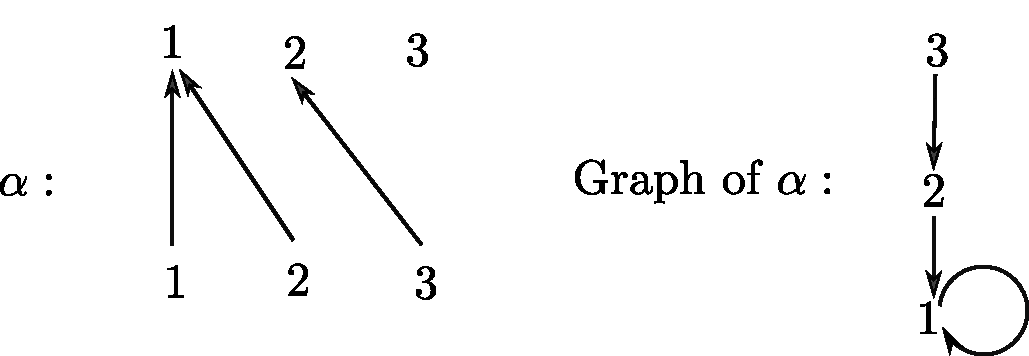
\includegraphics[scale=.4]{graph-of-alpha}
\end{center}
Consider the function
\begin{align*}
\ranked{\reduce k \Sigma^k \to \reduce 2 (\reduce {k-1} \Sigma^{k-1}\otimes \Sigma)}
\end{align*}
which acts as in the following picture
\begin{center}
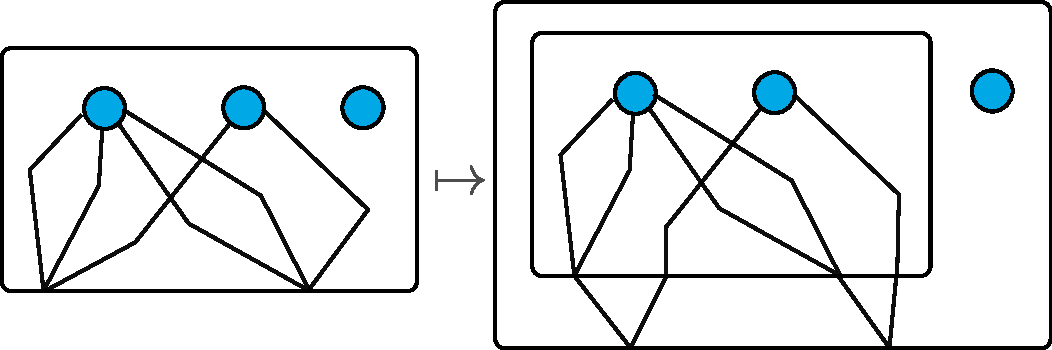
\includegraphics[scale=.4]{connected-alpha-hom}
\end{center}
If we inject both $\ranked{\reduce {k-1} \Sigma^{k-1}}$ and $\ranked{\Sigma}$ into $\rDelta\eqdef\ranked{\reduce {k-1} \Sigma^{k-1}+\Sigma}$, we get a term in the matrix power $\mati 2 \rDelta$. Note that the twists of such elements are the constant 1. We can then apply the unfolding function for constant-twists inputs
\begin{align*}
\ranked{\tmonad \mati 2 \Delta \to \mati 2 {\tmonad \Delta}}
\end{align*}
We can decompose the term $\tmonad \rDelta$ into  $\ranked{(\tmonad \reduce {k-1} \Sigma^{k-1})\odot \Sigma}$, by analyzing its structure. Now we can apply the induction hypothesis to unfold  $\ranked{\tmonad \reduce {k-1} \Sigma^{k-1}}$ into $\ranked{\reduce {k-1} (\tmonad \Sigma)^{k-1}}$. By applying the prime functions which permute the fold with the tensor product then increase the fold, we obtain the desired term.
\end{proof}


\subsubsection{Term unfolding for homogeneous inputs}
\label{subsec:something-homo-unfold}
we say that a term $ t \in \tmonad \mati k \rSigma$ is homogeneous if for every two internal branches $b_1, b_2$ having twists $\alpha_1, \alpha_2$ respectively and such that $b_2$ is a child of $b_1$, we have that
\begin{align*}
\alpha_1\alpha_2=\alpha_1
\end{align*}

The rest of this section is devoted to proving the following lemma. 

\begin{lemma}\label{lem:homo-2-twist}
    Let $k \in \set{1,2,\ldots}$. There is a derivable operation 
    \begin{align*}
        \ranked{f : \tmonad \mati k \rSigma \to \mati k {(\tmonad \Sigma)} }
        \end{align*}      
which coincides with term unfolding for all inputs which are homogeneous.
\end{lemma}

\begin{lemma}\label{lem:decomp-twist-2}
Let $\alpha:[1,k]\to [1,k]$ and $\beta:[1,k]\to [1,k]$ be two monotone functions such that
\begin{align*}
\alpha\beta=\alpha.
\end{align*}
 If the graph of $\alpha$ is not weakly connected, then so is the graph of $\beta$. Moreover, if $m\in \set{1,\dots, k}$ is such that 
\begin{align*}
\alpha[1,m] \subseteq [1,m]  \text{ and } 
\alpha[m+1,k]\subseteq [m+1,k]
\end{align*}
then we have also 
\begin{align*}
\beta[1,m]\subseteq [1,m] \text{ and }
\beta[m+1,k]\subseteq [m+1,k]
\end{align*}

 If the graphs of $\alpha$ and $\beta$ are both weakly connected, then  $\alpha$ and  $\beta$ are both constant functions.
\end{lemma}

\begin{proof}[Proof of Lemma~\ref{lem:homo-2-twist}]
We proceed by induction on $k$. The base case, ie when $k=1$ is realized by the untwist prime function. Let us treat the inductive case. First, we factorize our term in such a way that in each factor, either all the internal twits are weakly connected, or all of them are not weakly connected. To realize this factorization, it is enough to detect the first nodes (that is the closest to the root) where the twist becomes not weakly connected. Indeed, by Lemma\ref{lem:decomp-twist-2}, we know that the twits of the sub-tree rooted in such nodes are all not weakly connected. To detect these node, the following prime function is of particular interest
\begin{center}
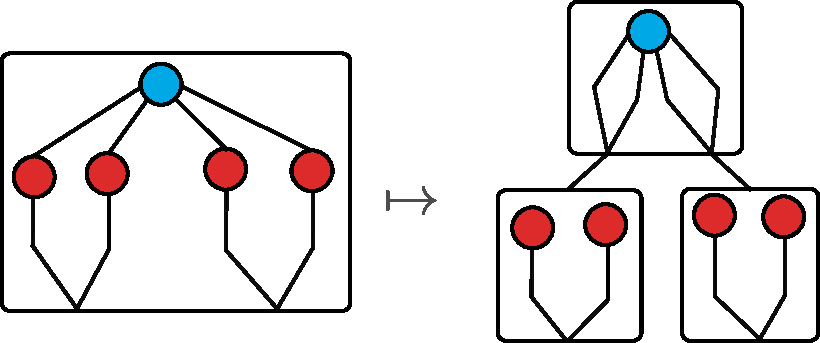
\includegraphics[scale=.4]{last-prime-function}
\end{center}
If we analyze this factorization, it has the form $\ranked{\tmonad \mati k \Sigma \odot \tmonad \mati k \Sigma}$, where the root contains only connected internal twists and the leaves only weakly connected internal twists. By Lemma~\ref{lem:decomp-twist-2}, we know that the internal twists of the root  are constant, and that in each leave, there is an integer $m$ such that every internal twist $\alpha$ satisfies
\begin{align*}
\alpha[1,m] \subseteq [1,m]  \text{ and } 
\alpha[m+1,k]\subseteq [m+1,k].
\end{align*}
To unfold the root, we apply Proposition\ref{lem:constant-twist}. To unfold each leave, we proceed by induction, in the exact same way as the non-connected case in the proof of Proposition~\ref{lem:homo-twist}. Finally to untwist the whole term, we apply the prime shallow unfold function. 
\end{proof}
